This chapter describes the user interface as well as some technical details of the implementation of the system. 
\section{User Interface}
The user interface (UI) between the user and the robot appears as a chat application. Figure \ref{fig:chatWindow} illustrates a text box of rules at first, followed by a box of chat dialogue and the message bar. User has 2 ways to interact: either texting or speaking (by using the \tit{Use Voice} button). 
\begin{figure}[tb]
	\centering
	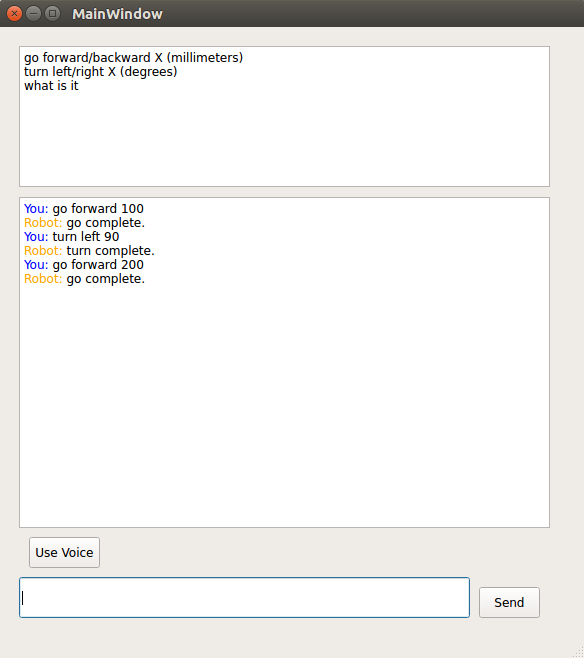
\includegraphics[width=0.8\hsize]{./figures/chatWindow}
	\caption{The chat window of the UI. There is a text box for reminding the rules of commands, followed by a text box of chat dialogue and the message bar.}
	\label{fig:chatWindow}
\end{figure}

The UI is coded using PyQt - one Python binding for Qt cross-platform GUI. The backend behind is Python code because the robot SDK is based on Python3. Beside the real Cozmo robot, I provided a simple robot simulator that can draws the movement commands (figure \ref{fig:simulator}). This simulator is programmed using Turtle module in Python.


\begin{figure}[!htb]
	\centering
	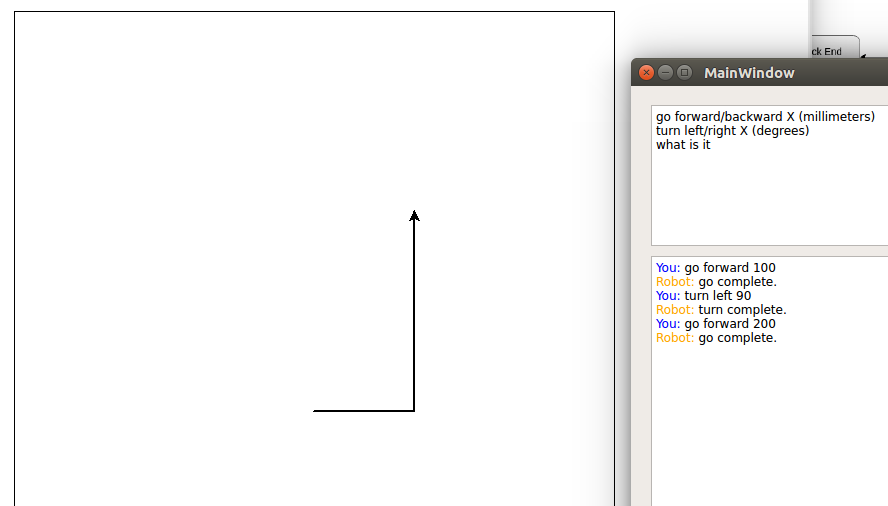
\includegraphics[width=0.8\hsize]{./figures/simulator}
	\caption{Turtle module draws the movement commands. This is useful for testing the system when we don't have a real Cozmo robot.}
	\label{fig:simulator}
\end{figure}

The overview of the system is described in figure \ref{fig:UIdesign}. The left right arrows are used to indicate the interaction between blocks. For example: User sends commands via User Interface and gets responses from here too.

\begin{figure}[!htb]
	\centering
	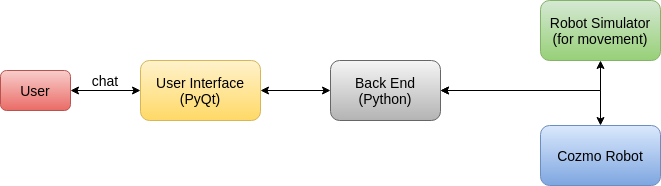
\includegraphics[width=1.0\hsize]{./figures/UIdesign}
	\caption{Overview of the system.}
	\label{fig:UIdesign}
\end{figure}

\section{The Cozmo Robot}
\label{sec:Cozmo}

Cozmo (figure \ref{fig:cozmo}) is a great robot from Anki \cite{AnkiOfficial:2017}. Beside concise movement ability, my Cozmo also has a built-in QVGA camera with frame rate 15fps \cite{cozmoTech}. Eventhough the camera is not good, it still gives us acceptable images and helps us avoid building a robot from scratch, which can be time consuming.

\begin{figure}[!htb]
	\centering
	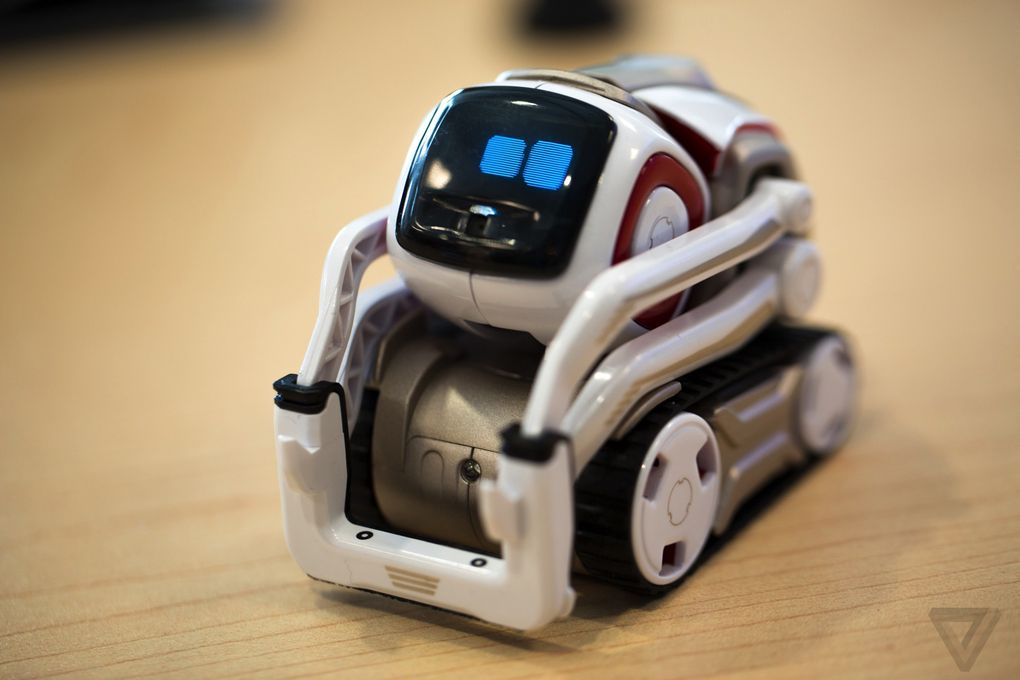
\includegraphics[width=0.8\hsize]{./figures/cozmo}
	\caption{Cozmo robot that has concise movement, built-in QVGA camera as well as other features (LED screen, etc.). Image source: theverge.com}
	\label{fig:cozmo}
\end{figure}

\subsection{Camera Sensor}
\label{subsec:camInfo}
 As stated above, my Cozmo has a QVGA (resolution $320 \times 240$) camera built-in with frame rate 15fps. \tit{Please note that Anki seems to understand this limitation and decide to upgrade the camera sensor to a VGA (resolution $640 \times 480$) camera with 30 fps in the recent Cozmo robots.}. Here are a few details about the camera sensors:
 \begin{itemize}
 	\item focal length in x axis: 292.84 (pixels)
 	\item focal length in y axis: 292.84 (pixels)
 	\item field of view in x axis: $57^{\circ}$
 	\item field of view in y axis: $44^{\circ}$
 	\item center of image in x axis: 161.09 (pixels)
 	\item center of image in y axis: 128.56 (pixels)
 \end{itemize}
Figure \ref{fig:cozmoRealImg} shows images captured by Cozmo. Beside the low resolution, we can also see light intensity flickering problem with photos taken under fluorescent light sources.

\begin{figure}[!htb]
	\centering
	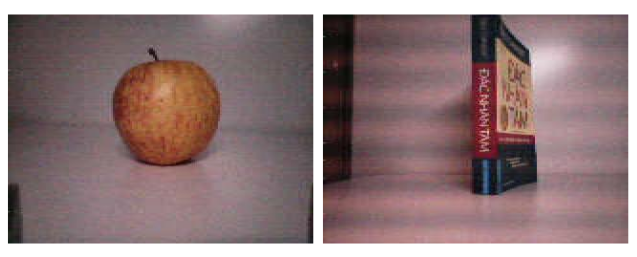
\includegraphics[width=1.0\hsize]{./figures/cozmoRealImg}
	\caption{Images taken from Cozmo's camera. \tbf{Left:} Photo of an apple is shown. We can see that the image is noisy and its resolution is low. \tbf{Right:} Photo of a book is shown. We can see the light intensity flickering problem for images taken under fluorescent light sources (the horizontal stripes in the image).}
	\label{fig:cozmoRealImg}
\end{figure}


 \subsection{Communication}
The connection between Cozmo and our system is illustrated in figure \ref{fig:CozmoConnect}. Cozmo will connects to a mobile device (that has Cozmo application installed) via its own wifi. In my setup, the mobile device is an IPad. Then it is connected to our system (the computer) via a USB cable. Linux machines now can access iOS device (such as IPhone, IPad) through \tit{libimobiledevice} \cite{libimobiledevice}. The following steps summarize the process:
\begin{enumerate}
	\item Connect the mobile device to the system via USB.
	\item Start Cozmo and connect the mobile device to the Wifi of Cozmo.
	\item Enable SDK mode in Cozmo application on the mobile device.
	\item Launch our program and start using it.
\end{enumerate}
\begin{figure}[!htb]
	\centering
	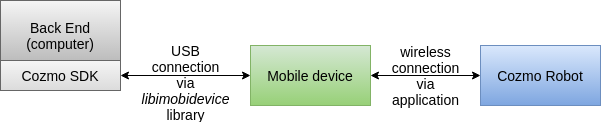
\includegraphics[width=0.9\hsize]{./figures/CozmoConnect}
	\caption{Cozmo connects with the system via a mobile device that has Cozmo app installed.}
	\label{fig:CozmoConnect}
\end{figure}

\section{The Reader and Action classes}
Given the text command, we have a Reader instance that will do the preprocessing and extract information from it (discussed in subsection \ref{sec:InfoExt}). Based on each intents, we map it into an instance of corresponding Action. These Action classes are implemented to control the robot and the simulator to act correspondingly. Figure \ref{fig:readerAction} illustrates this process. 

\begin{figure}[!htb]
	\centering
	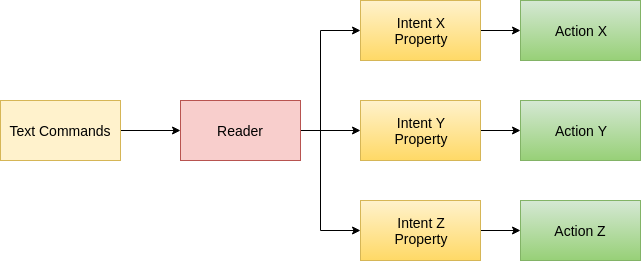
\includegraphics[width=0.9\hsize]{./figures/readerAction}
	\caption{Commands are parsed via a Reader object. Then they are handled accordingly via their corresponding Action objects.}
	\label{fig:readerAction}
\end{figure}

\section{Threading}
There are a few scenarios where we need to use threading in order to avoid freezing the user interface:
\begin{itemize}
	\item time to record the audio command: which can vary from 3 to 15 seconds
	\item speech recognition task that sends audio command over the internet, time for doing this task depends to your inernet connection. However, in practice it's quite fast because the recorded file is about 100Kb.
	\item classify image: ask robot to take a photo, and pass this image through a neural network model (discussed in subsection \ref{sec:transferLearning}) to get prediction of class probabilities.
\end{itemize}

\begin{figure}[!htb]
	\centering
	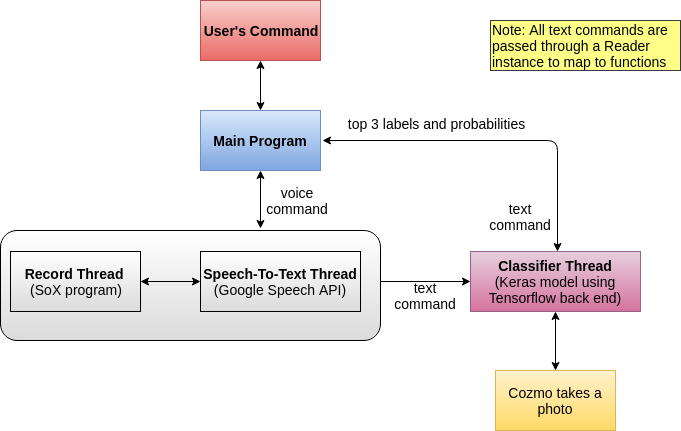
\includegraphics[width=0.9\hsize]{./figures/threads}
	\caption{Threading}
	\label{fig:threads}
\end{figure}

Figure \ref{fig:threads} illustrates the threading structure of the program. Initially, the main program will run these threads in background. Then, whenever user's command needs to use them, these threads are waken up to do their jobs. Note that record thread always works together with speech recognition thread. The idea of seperating them in 2 threads is for further development when we could probably try other speech recognizers.

\section{Dataset}
TODO: explain how many dataset is used, how it is collected and structured

\subsection{Dataset Characteristic}
Images from ImageNet are taken from many sources and some of them can be really confusing. For example, image in category \tit{Apple} can contain also other fruits (figure \ref{fig:imhard1}). Some of them are just simply difficult because the label is not the main content of the picture (figure \ref{fig:imhard2}). However, this diversity makes the system more flexible and robust at test time because in practice, we can have objects mixed together or not in the center of the image. Therefore, I chose to keep this characteristic.

\begin{figure}[!ht]
	\centering
	\begin{minipage}[t]{0.45\linewidth}
		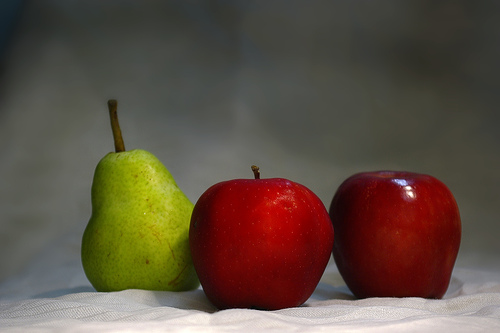
\includegraphics[scale=0.37]{./figures/imhard1}
		\caption{This image belongs to class \tit{Apple} but contains also a \tit{Pear}.}
		\label{fig:imhard1}
	\end{minipage}
	\quad
	\begin{minipage}[t]{0.45\linewidth}
		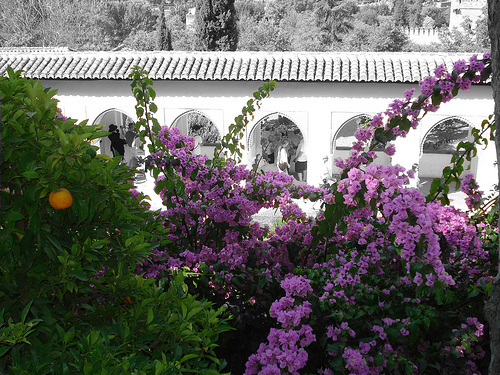
\includegraphics[scale=0.35]{./figures/imhard2}
		\caption{This image belongs to class \tit{Orange} but there is only a small orange on the left side.}
		\label{fig:imhard2}
	\end{minipage}
\end{figure}

\section{Data Preprocessing and Augmentation}
Commonly, there are two principal types of preprocessing data: \tit{mean subtraction} and \tit{normalization}. Preprocessing data normally helps training faster and empowers activation functions such as ReLU ($f(x) = max(x, 0)$).

\subsection{Mean Subtraction}
Mean subtraction make data zero-centered (middle plot in figure \ref{fig:prepro1}). First, we calculate the mean image of all the \tbf{training images}, across the three color channels. Then, we subtract all the images (in training, validation and test set) by this mean. 
\subsection{Normalization}
Normalize data is to scale data to a fixed range $[-r, +r]$ where range $r$ is normally $1$. To do so, we calculate the standard deviation image of all the \tbf{training images}, across the three color channels. Then we divide all the images (in training, validation and test set) by this standard deviation. This is illustrated in right plot of figure \ref{fig:prepro1}. Note that the pixel value is already in range $[0, 255]$ hence normalization is not required for image.

\begin{figure}[tb]
	\centering
	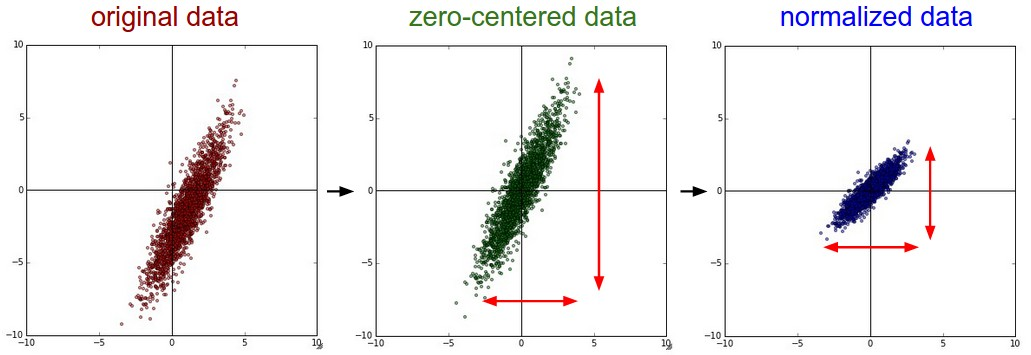
\includegraphics[width=0.9\hsize]{./figures/prepro1}
	\caption{Left: original 2D input data. Middle: subtracted mean data. Right: subtracted mean and normalized data. \tit{Image courtesy of Andrej Kaparthy \cite{cs231n}.}}
	\label{fig:prepro1}
\end{figure}

\subsection{Image Augmentation}
There are many ways to augment our dataset: flipping, rotating, cropping, distorting images, adding noise, etc. Becase of the limited computation resource, I only used the following augmentation techniques (figure \ref{fig:augment1}):
\begin{itemize}
	\item add a bit of noise on original image (sub-image 4)
	\item flip image vertically (sub-image 2) and add a bit of noise (sub-image 5)
	\item flip image vertically (sub-image 3) and add a bit of noise (sub-image 6)
\end{itemize}
\begin{figure}[bh!]
	\centering
	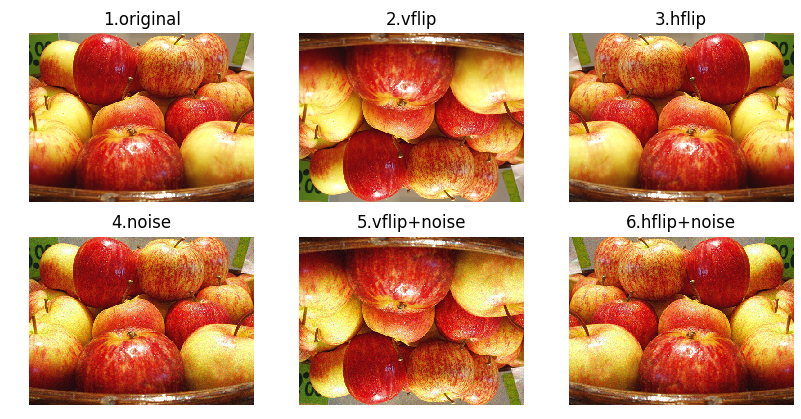
\includegraphics[width=0.8\hsize]{./figures/augment1}
	\caption{Augmented images: (1) original, (2) vertical flip, (3) horizontal flip, (4) noise, (5) verticalf lip plus noise, (6) horizontal flip plus noise.}
	\label{fig:augment1}
\end{figure}


TODO: add details about github, commits, fork, etc.